\documentclass[11pt]{exam}
\usepackage[empty]{fullpage}
\usepackage{amsmath,amssymb}
\usepackage{colortbl}
\usepackage{subfig}
\usepackage{multicol}
\usepackage{tikz,pgfplots}
\usepgfplotslibrary{statistics}
\usepackage{color,comment,soul}

\newcommand{\blank}[1]{\underline{\hspace*{#1}}}
\newcommand{\ds}{\displaystyle}
\newcommand{\mymod}{~\mathrm{mod}~}


\begin{document}
\graphicspath{{/home/brian/Dropbox/HSC/Spring16/Math111/}}

\subsubsection*{Midterm 2 Review - Math 243}

\begin{questions}
%%%%%%%%%%%%%%%%%
%%% Problem 1 %%%
%%%%%%%%%%%%%%%%%
\question Determine the type of the equilibrium (sink, source, spiral sink, spiral source, saddle, or center) at the origin for each of the following linear systems. 
\begin{parts}
\part $\ds{\frac{dX}{dt} = \left[ \begin{array}{cc} 2 & 0 \\ 0 & 3 \end{array} \right] X}$ \\ \\
\part $\ds{\frac{dY}{dt} = \left[ \begin{array}{cc} -1 & -5 \\ 4 & -2 \end{array} \right] Y}$ \\ \\
\part $\ds{\frac{dZ}{dt} = \left[ \begin{array}{cc} 2 & 3 \\ 1 & 0 \end{array} \right] Z}$ \\ \\
\end{parts}

\question Show that $\begin{bmatrix} 2 \\ i \end{bmatrix}$  is an eigenvector for the matrix $A = \begin{bmatrix} 0 & 4 \\ -1 & 0 \end{bmatrix}$. What is the corresponding eigenvalue? 
\vfill

\question Use the eigenvalue and eigenvector from the previous problem to find the general solution of the system
$$\dfrac{d\mathbf{x}}{dt} = \begin{bmatrix} 0 & 4 \\ -1 & 0 \end{bmatrix} \mathbf{x}.$$

\vfill

\question Consider the one-parameter system $\dfrac{d\mathbf{y}}{dt} = \begin{bmatrix} 1 & a \\ 1 & 3 \end{bmatrix} \mathbf{y}$. Use the trace and determinant to find the values of $a$ where the type of equilibrium changes.  Describe in words how the type of equilibrium depends on $a$. 
\vfill

\newpage
\question Find the eigenvalues for the matrix $\begin{bmatrix} 2 & -6 \\ 2 & -3 \end{bmatrix}$.  For each eigenvalue, find a corresponding eigenvector. 
\vfill

\question Use the eigenvectors and eigenvalues from the last problem to find the general solution of the linear system
$$\dfrac{dx}{dt} = 2x - 6y,$$
$$\dfrac{dy}{dt} = 2x - 3y.$$
\vfill


\question The system 
$$\dfrac{dx}{dt} = x - 2y,$$
$$\dfrac{dy}{dt} = 3y$$
is partially decoupled. Suppose that $x(0) = 1$ and $y(0) = 2$.  Solve this initial value problem by solving for $y(t)$ first, and then use $y(t)$ to find $x(t)$.  
\vfill

\question The previous example can be expressed using matrix notation as $\mathbf{x}' = A \mathbf{x}$ where $A = \begin{bmatrix} 1 & -2 \\ 0 & 3 \end{bmatrix}$.  It turns out that 
$$e^{At} = \left[\begin{matrix}e^{t} & - e^{3 t} + e^{t}\\0 & e^{3 t}\end{matrix}\right].$$
Use this to solve the initial value problem above. 
\vfill

\newpage
\question The following direction fields represent linear systems $\mathbf{x}' = A\mathbf{x}$.  Match each direction field with the correct matrix from the options below. \\
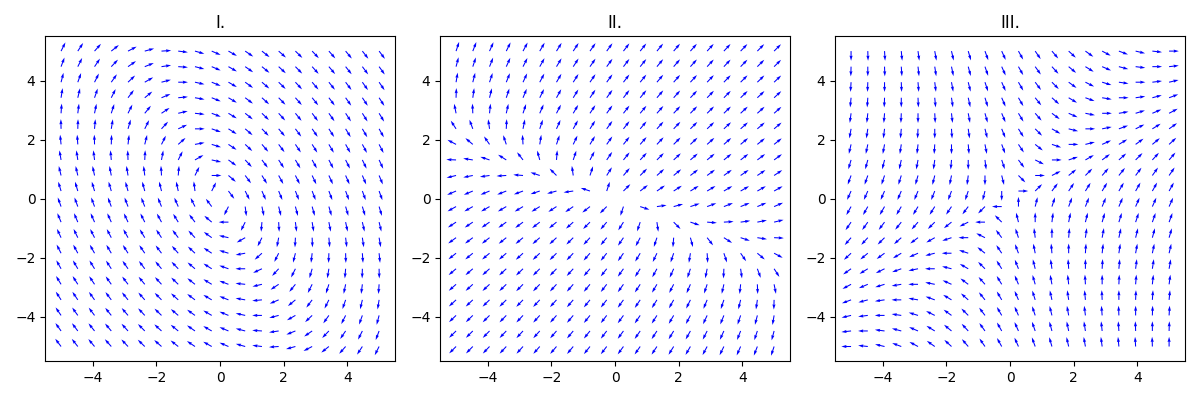
\includegraphics[scale=0.55]{reviewDirectionFields.png}

\begin{oneparchoices}
\choice $\begin{bmatrix} 2 & 3 \\ 1 & 4 \end{bmatrix}$ \hspace{0.5in}
\choice $\begin{bmatrix} 1 & 2 \\ -3 & -1 \end{bmatrix}$ \hspace{0.5in}
\choice $\begin{bmatrix} -4 & 0 \\ 1 & -3 \end{bmatrix}$ \hspace{0.5in}
\choice $\begin{bmatrix} 1 & 1 \\ 2 & -2 \end{bmatrix}$ 
\end{oneparchoices}
\vfill


\question Find the general (real-valued) solution to the system 
$$\dfrac{dx}{dt} = x + 3z,$$
$$\dfrac{dy}{dt} = -3y,$$
$$\dfrac{dz}{dt} = 3x + z.$$
\vfill
\vfill

\question Find the solution of the last problem that satisfies the initial condition
$$x(0) = 5,$$
$$y(0) = 2,$$
$$z(0) = -1.$$
\vfill
\vfill

\question The system $\dfrac{dX}{dt} = \begin{bmatrix} -5 & 3 \\ -3 & 1 \end{bmatrix} X$ has $\lambda = -2$ as a repeated eigenvalue.  What is the solution to the system with initial condition $X(0) = \begin{bmatrix} -1 \\ 1 \end{bmatrix}$?
\vfill
\vfill


\end{questions}

\end{document}
